\documentclass[10pt,a4paper]{report}
\usepackage[utf8]{inputenc}
\usepackage{amsmath}
\usepackage{amsfonts}
\usepackage{amssymb}
\usepackage{listings}
\usepackage{struktex}

\usepackage{tikz}
%%%%<
%\usepackage{verbatim}
%\usepackage[active,tightpage]{preview}
%\PreviewEnvironment{tikzpicture}
%\setlength\PreviewBorder{5pt}%
%%%%>

\usetikzlibrary{arrows,%
                shapes,positioning}

\begin{document}
\chapter{Durchmusterung der Geotiff Daten und Auffinden der Landebahnen}
Die Durchmusterung der Geodaten wurden in einer eigenen statischen Library gekapselt ($plane\_library.a$). Innerhalb dieser Library finden sich alle Algorithmen, die zum Auffinden der Landebahnen benötigt werden. Für den Aufrufer ist die Implementation komplett unsichtbar und gekapselt. Alle funktionalen Requirements werden von dieser Library übernommen.


\section{Interface der Library}

Die Parameter des Interfaces sind im Listing \ref{interface} beschrieben.

\begin{lstlisting}[caption=Interface Beschreibung, label=interface]
int search_for_planes(const tileData *actualTile, 
GeoTiffHandler *myGeoTiffHandler, 
float heading, float minLength, float width, int commSocket,
const json *taskDescription, float noDataValue , rectSize pixelSize );
\end{lstlisting}

Die einzelnen Aufrufparameter und deren funktionale Eigenschaft sind in Tabelle~\ref{beschreibungparameter} aufgezeigt.

\begin{table}[htb]
\centering
\begin{tabular}{|p{4.5cm}|p{10cm}|}
\hline 
Parameter & Funktion \\ 
\hline 
*actualTile & Zeiger auf das Geo Kartenobjekt mit den einzelnen Höhendaten \\ 
\hline 
*myGeoTiffHandler & Zeiger auf eine Instanz eines GeoTiffHandler Objekts, 
welches diverse Funktionen zur Umrechnung, Konvertierung etc. im GeoTiff Format unterstützt \\ 
\hline 
heading & Durchmusterungswinkel für die Landebahnen $0^\circ$ => Nord-Süd Achse \\ 
\hline 
minLength & minimale geforderte Länge der Landebahn \\ 
\hline 
width & Breite der geforderten Landebahn \\ 
\hline 
commSocket & Socket für das abspeichern gefundener Landebahnen in der Mongo DB\\ 
\hline 
*taskDescription & Taskbeschreibung, um die gefundene Bahn korrekt in Mongo abzulegen \\ 
\hline 
noDataValue & Zahlenwert für undefinierte Kartenpunkte \\ 
\hline 
pixelSize & Auflösung der Rasterpunkte in [m]\\
\hline 

\end{tabular} 
\caption{Beschreibung der Aufrufparameter Funktionalität}\label{beschreibungparameter}
\end{table}

\section{logischer Ablauf innerhalb der Landebahn Erkennung}

Der logische Ablauf ist schematisch im Nassi-Shneiderman-Diagramm~\ref{nasshnlogisch} dargestellt.

\clearpage
\begin{struktogramm}(100,200)\label{nasshnlogisch}
  \assign{Initialisisierung $tile\_worker$ Objekt}
  \assign{Berechne winkel-, steigungs- und holprigkeitsabhängige Parameter}
\forallin{Für alle Startpunkte einer Landebahn in gegebener Richtung (Thread Pool)}
\assign{wähle den nächsten Punkt}
\ifthenelse[15]{1}{1}
{kurzreichweitige Steigung zum Vorgänger OK?}{\sTrue}{\sFalse}
\ifthenelse[17]{1}{6}
{checke Holprigkeit in Querrichtung}{\sTrue}{\sFalse}
\change
\ifthenelse[25]{1}{1}
{ist die aktuelle Landebahn länger als die Mindestlänge}{\sTrue}{\sFalse}
\assign{Suche die beste Landebahn mit Mindestlänge}
\assign{Speichere beide Landebahnen in der Mongo DB}
\assign{starte eine neue Landbahn mit aktuellem Punkt}
\change
\assign{starte eine neue Landbahn mit aktuellem Punkt}
\ifend
\ifend
\change
\ifthenelse[30]{1}{1}
{ist die aktuelle Landebahn länger als die Mindestlänge}{\sTrue}{\sFalse}
\assign{Suche die beste Landebahn mit Mindestlänge}
\assign{Speichere beide Landebahnen in der Mongo DB}
\assign{starte eine neue Landbahn mit aktuellem Punkt}
\change
\assign{starte eine neue Landbahn mit aktuellem Punkt}
\ifend
\assign{starte eine neue Landbahn mit aktuellem Punkt}
\ifend
\forallinend
\end{struktogramm}

\clearpage
\section{Initialisierung}

Die Initialisierung erzeugt zunächst ein $tile_worker$ Objekt und initialisiert die Instanzvariablen mit den bei der Objekterzeugung angegebenen Durchmusterungscharakteriska wie maximale erlaubte Steigung, Varianz, minimale Landebahnlänge.
Mit dem Aufruf von $check_steigungen$ werden dann die optimalen Schrittvektoren und die Startkoordinaten des Durchmusterungsvorgangs bestimmt.
Die optimalen Durchmusterungsvektoren sind winkelabhängig. Die Idee hierbei ist, dass in Abhängigkeit der Auflösung diese Vektoren so initialisiert werden, dass alle möglichen Landebahnen gefunden werden. Dies führt dazu, dass bestimmte Winkel beim Durchmustern dichtere Landebahnen abtasten können. Somit wird sichergestellt, dass jede Landebahn mindestens einmal untersucht wird.
Zusätzlich dazu werden dann orthogonale Vektoren aus den Schrittvektoren abgeleitet, die zum Durchmustern in orthogonaler Richtung (Landebahnbreite) benutzt werden.
Anhand der gegebenen Kartenauflösung und Schrittvektoren kann dann bestimmt werden, wie viele aufeinander folgende Punkte mindestens benötigt werden, damit die Landebahn die Mindestlängenvoraussetzung erfüllt.
Entsprechendes gilt natürlich auch für die Breite der Bahn.
Anschließend werden dann die Startpunkte der Durchmusterung bestimmt.
Diese sind abhängig vom Durchmusterungswinkel. 
Für Winkel, die ein vielfaches von 90 betragen, wird einfach eine Seite des Quadranten abgeschritten. Wird eine Bahn z.B. in $y$-Richtung abgetastet, wird der Abzissenwert inkrementiert / dekrementiert und erneut in $y$-Richtung abgeschritten, bis der Rand der Kachel erreicht wird.
Bei Winkeln, die nicht einem Vielfachen von 90 entsprechen, werden sukzessiv sowohl Abszisse als auch Ordinate abgeschritten und das Terrain in Diagonaler Richtung durchmustert. 
Einige grafische Beispiele sind in Diagramm ... angegeben.

\begin{figure}
\centering
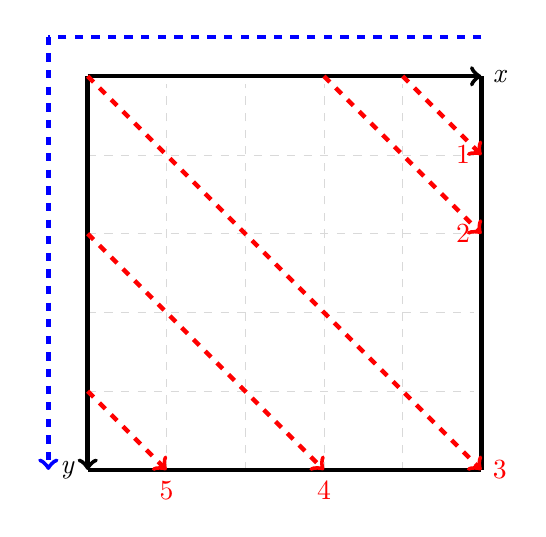
\begin{tikzpicture}
\draw[help lines, color=gray!30, dashed] (0,0) grid (4.9,4.9);
\draw[->,ultra thick] (0,5)--(5,5) node[right]{$x$};
\draw[->,ultra thick] (0,5)--(0,0) node[left]{$y$};

\draw[-,ultra thick] (5,5)--(5,0) node[left]{};
\draw[-,ultra thick] (0,0)--(5,0) node[right]{};

\draw[->,ultra thick,dashed,red] (4,5)--(5,4) node[left]{$1$};
\draw[->,ultra thick,dashed,red] (3,5)--(5,3) node[left]{$2$};
\draw[->,ultra thick,dashed,red] (0,5)--(5,0) node[right]{$3$};

\draw[->,ultra thick,dashed,red] (0,3)--(3,0) node[below]{$4$};

\draw[->,ultra thick,dashed,red] (0,1)--(1,0) node[below]{$5$};

\draw[-,ultra thick,dashed,blue] (5,5.5)--(-0.5,5.5) node[left]{};
\draw[->,ultra thick,dashed,blue] (-0.5,5.5)--(-0.5,0) node[left]{};
\end{tikzpicture}
\caption{Verschiebung des Startpunkts der Landebahndurchmusterung in diagonaler Richtung. Hier NNO nach SSW.}
\end{figure}


\begin{figure}
\centering
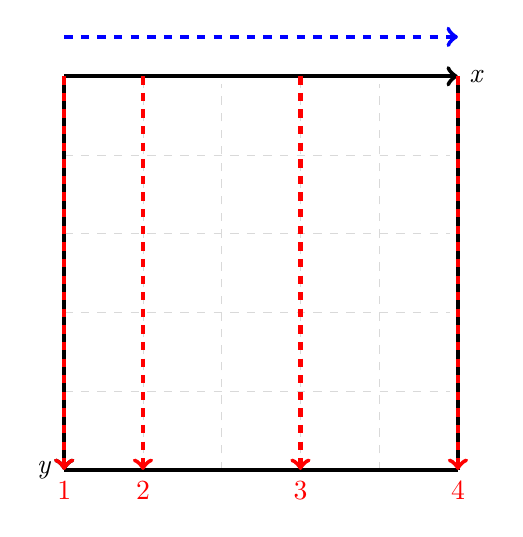
\begin{tikzpicture}
\draw[help lines, color=gray!30, dashed] (0,0) grid (4.9,4.9);
\draw[->,ultra thick] (0,5)--(5,5) node[right]{$x$};
\draw[->,ultra thick] (0,5)--(0,0) node[left]{$y$};

\draw[-,ultra thick] (5,5)--(5,0) node[left]{};
\draw[-,ultra thick] (0,0)--(5,0) node[right]{};

\draw[->,ultra thick,dashed,red] (0,5)--(0,0) node[below]{$1$};
\draw[->,ultra thick,dashed,red] (1,5)--(1,0) node[below]{$2$};
\draw[->,ultra thick,dashed,red] (3,5)--(3,0) node[below]{$3$};
\draw[->,ultra thick,dashed,red] (5,5)--(5,0) node[below]{$4$};


\draw[->,ultra thick,dashed,blue] (-0,5.5)--(5,5.5) node[left]{};
\end{tikzpicture}
\caption{Verschiebung des Startpunkts der Landebahndurchmusterung in diagonaler Richtung. Hier N nach S.}
\end{figure}
\section{Parallelverarbeitung mittels pthreads zum Finden der Landebahnen}

Die Parallelverarbeitung arbeitet nach einem Task-Workermodell, welches mit einem Semaphor gesteuert wird. Jeder Startpunkt, der auf einem Kartenrand liegt, ist hier als ein Task anzusehen. Das Semaphor dient dazu, die gleichzeitige Anzahl der Threads zu steuern und zu kontrollieren. Dies dient zum einen Untersuchungszwecken, um festzustellen, die der Speedup bei Variation der Threads ist. Weiterhin würde eine zu hohe Zahl an an Threads die ausführende Maschine in extreme Ressourcenknappheit bringen können.
Das Workerobjekt kontrolliert mit einem mutex die Herausgabe von Startwerten. In einem kritischen Bereich wird durch Inkrementierung des Startpunktes ein neuer Startpunkt generiert, der an einen Worker als Form eines abzuarbeitenden Task herausgegeben wird. Dieser kritische Bereich, der dafür sorgt, dass jeder Startpunkt auch nur wirklich einmal herausgeben wird, stellt somit auch das Bottleneck der Parallelverarbeitung dar. So lange die Anzahl der Punkte pro Bahn und die Berechnungszeit, die ein Thread benötigt, um die Bahn in der vorgegebenen Richtung abzuscannen und die zur Bahn gehörigen Parameter wie Varianz etc. zu berechnen größer ist als die Zeit, die vergeht, bis der Thread wieder in der Warteschlange zum Erhalt eines neuen Startwert aufläuft, sollte dieses Bottleneck gering sein.
Zudem ist zu beachten, dass natürlich nicht alle Landebahnen gleich lang sind. So lange der Startpunkt in der Nähe einer Kartenecke ist und die Durchmusterungsrichtung nur wenige Punkte bis zum Kartenrand umfasst, wird die Durchmusterung schnell vorbei sein und ein neuer Startwert benötigt werden. 

\section{Detaillierte Beschreibung des Suchalgorithmus}

Ausgehend vom jeweiligen Startpunkt wird mittels p\_thread\_create ein neuer Thread erzeugt und die Funktion void *thread\_data::check\_single\_plane(void *x\_void\_ptr) als Startroutine mitgegeben. Innerhalb dieses erzeugten Threads existiert eine while Schleife, die solange true returniert, wie noch nicht alle Startpunkte an Threads ausgeben wurden.
Innerhalb einiger verschachtelten Bedingungen wird überprüft, ob der betrachtete Geopunkt tatsächlich Höheninformationen hat und ob die Steigung zu seinem unmittelbaren Vorgänger innerhalb des erlaubten Bereiches liegt.
Trifft dies zu, so ist noch die Steigung benachbarter Punkte in orthogonaler Richtung zu betrachten. Sind all diese Kriterien erfüllt, wird der betrachtete Geopunkt in eine Liste an gültigen Punkten aufgenommen. Diese Prozedur wird so lange wieder holt, bis ein Kriterium nicht mehr erfüllt ist oder der Kartenrand erreicht ist.
Ist eines dieser Abbruchkriterien erfüllt, wird überprüft, ob das Ensemble aneinanderhängender Punkte die Mindestlänge der geforderten Landebahn erfüllt.
Dann wird eine Subroutine find\_best\_planes() aufgerufen, welche innerhalb der gefunden Liste an zusammenhängenden Punkten zwei Landebahnen ermittelt. Zum einen wird die längste Bahn, die das Steigungskriterium erfüllt ermittelt und des weiteren die Landebahn, die die geringste Varianz aufweist und trotzdem noch die geforderte Mindestlänge erreicht. 
Beide Bahnen werden dann, so fern vorhanden, in einer Mongo DB abgelegt.

\section{Klassen und Objekte}

In der $plane\_library.a$ werden mehrere Klassenimplementationen verwendet, um objektorientiert zu einer vereinfachten Problemlösung zu gelangen.
Die zentrale Klasse ist dabei die $tile_worker$-Klasse. In ihr werden wichtige Membervariablen zu den parametriesierten Rahmenbedingungen verwaltet und das Threading mittels p\_thread abgehandelt. Die Klasse $landing_plane$ beschreibt ein Hilfsobjekt, in dem gefundene Landebahnobjekte via Startpunkten, Steigung und Varianz beschrieben wird.
Das Threading selbst hat eine sehr schlanke $thread_data$-Klasse, welche in einer "friend"-Beziehung zum $tile_worker$ steht und sich ausschließlich mit der Parallelausführung beschäftigt.
Der $tile-manager$ ist eine Klasse, die ausschließlich zu Debug- und Entwicklungszwecken zum Bau eines Standalone Binaries benötigt wird.
Für den produktiven Einsatz ist sie obsolet.


\section{Verwendete Datenstrukturen}

Die wichtigsten Datenstrukturen, die während der Durchmusterung benötigt werden, sind das übergebene Kachelobjekt, ein Objekt zur Verwaltung der aktuell gefundenen zusammenhängenden Punkte, sowie den $tile_worker$, der die Threads kontrolliert und Durchmusterungsparameter kapselt. 

\subsection{Einfluss der Datenstrukturen auf die Performanz}

Die Container-Klasse des $tile_workers$ hat in seiner endgültigen Form keine komplexeren Datenstrukturen mehr. Sie beinhaltet lediglich Membervariablen einfacher Datentypen wie $double$ und $int$.
Innerhalb der Thread-Klasse findet sich eine lokale Variable $coordlist$, welche vom Typ $vector< pair<int,int> >$ ist.
Hier werden temporär aneinanderhängende Ketten von Landebahnpunktkoordinaten vorgehalten. Die gespeicherten Punkte sind dabei lediglich Referenzen auf das statische Kartenobjekt. Ohne dieses wären die Informationen bedeutungslos.
Der Vorteil des vector templates in C++ ist der optimierte random access, welcher in der Komplexizitätsklasse O(1) zu finden ist und die Verwaltung sehr komfortabel mittels Member-Funktionen vorgegeben ist.
Das Kachelobjekt selbst  stellt die Höheninformationen eines 2-dimensionalen Kartenausschnitts in einem linearen Array dar. Der Durchmusterungsalgorithmus benötigt allerdings einen Mappingmechanisumus eines 2-dimensionalen Punktes auf das eindimensionales Array.
Dies wird von der Funktion $access_single_element(int x, int y)$ bereitgestellt. Anhand der Information, wie viele Datenpunkte der Kartenausschnitt in $x$-Richtung beinhaltet, wird das Mapping auf das eindimensionale Array dargestellt. Im Falle einer Bereichsüberschreitung, wird $numeric_limits<float>::min()$ zurückgegeben.
Auch dieser Zugriff ist der Komplexitätsklasse O(1) zuzuordnen und unabhängig von Datengröße.

\begin{lstlisting}
float tile_worker::access_single_element(int x, int y)
{
  if (tile->width.x*y+x < tile->width.x*tile->width.y)
    return(tile->buf[tile->width.x*y+x]);
  else
   return numeric_limits<float>::min();

}
\end{lstlisting}

Dies führt dazu, dass der Speicherbedarf ausschließlich von der Anzahl der Datenpunkte in den Rohdaten abhängig ist. Für die Speicherallokierung werden insbesondere bei den C++ Templates vordefinierte default-Allokatoren genutzt, die man natürlich mit eigens definierten überladen könnte. Dafür gibt es bislang aber keinerlei Gründe.
 


\section{Bestimmung des Speedups in Abhängigkeit des Parallelisierunggrades}

Um den Speedup zu bestimmen, wurde analysiert, wie sich die Laufzeit mit zunehmender Anzahl an Threads verändert. So lange die Bearbeitung einer einzelnen Bahn viel länger dauert als die in der kritischen Sektion benötigte Zeit, um einen neuen Startpunkt zu bestimmen, sollten die Threads nicht blockiert sein.
Bei Winkeln, die ein vielfaches von $90$ betragen, sind alle Landebahnen gleich lang --- also sind gleich viele Punkte zu analysieren.
Bei Bahnen, die diagonal verlaufen, sind die ersten Bahnen kurz, nehmen dann in ihrer Länge zu, bis als Startpunkt die nächstliegende Ecke  erreicht ist, und nimmt dann in ihrer Länge wieder ab. Weiterhin ist zu beachten, dass je nach Topologie der Bahn unterschiedlich viele (im Grenzfall gar keine) geeigneten Flächen gefunden werden, die dann fein granular weiter untersucht werden müssen (längste und mit der kleinsten Varianz). So ist schwer vorhersagbar, wie lange die Einzellaufzeit eines Threads ist.
Für die zur Verfügung gestellten Kartendaten von Nordrhein-Westfalen sind die Laufzeiten in Abhängigkeit von Winkel und Threadanzahl in Tabelle x dargestellt. Das verwendete System zur Analyse war eine virtualisierte VM (Centos 7.0, xx CPUs, xx GB RAM) 

Eine weiterfhrende Analyse war aufgrund mangelnder Hardwareressourcen nicht möglich.


\section{Analyse mittels Profiler}

Mittels gproof wurde analysiert, welche Programmteile beim Auffinden der Landebahn die meiste Rechenzeit benötigen. Hierdurch kann kontrolliert werden, ob die vom Scheduler zur Verfügung gestellten Zeitscheiben auch effektiv innerhalb des Threadings genutzt werden können. 
Bei der Analyse zeigt sich, dass die Funktion, die die meiste Zeit in Anspruch nimmt, die Zugriffsfunktion auf die Geopunkte ist. Hier findet ein Random Memory access statt (2-Dimensionalität wird auf ein eindmensionales Array abgebildet).
Eine weitere zeitintensive Funktion stellt die Berechnung der Varianz sowie das Auffinden der längsten und der varianzminimalen Landebahn dar.
Diese Ergebnisse sind intuitiv zu erwarten.
Da beide Funktionen innerhalb des Threading aufgerufen werden, ist aus laufzeittechnischer Sicht eine optimale Lösung gefunden. 

\section{Einfluss von Compiler Direktiven (speziell Optimizer)}

Bevor Codeausführung mittels Parallelverarbeitung zur Beschleunigung gebacht werden soll, lohnt es sich meist, durch geeignete Compilerdirektiven die serielle Codeausführung zu beschleunigen.
Der Code wurde mit einem gcc Version xx devtoolset yx compiliert. Die Standardübersetzung ist dabei ohne eingeschalteten Optimizer. 
Durch die Benutzung des -O3 Optimizer Direktivs ist eine Codebeschleunigung von yx \% beobachtet worden. 
Eine Übersicht über die verwendeten Optimierungsschritte sind unter https://gcc.gnu.org/onlinedocs/gcc/Optimize-Options.html einzusehen.


%\begin{tikzpicture}[node distance   = 4 cm]
%  \useasboundingbox (-1,-1) rectangle (11,11); 
%  \tikzset{VertexStyle/.style = {shape          = circle,
%                                 ball color     = orange,
%                                 text           = black,
%                                 inner sep      = 2pt,
%                                 outer sep      = 0pt,
%                                 minimum size   = 24 pt}}
%  \tikzset{EdgeStyle/.style   = {thick,
%                                 double          = orange,
%                                 double distance = 1pt}}
%  \tikzset{LabelStyle/.style =   {draw,
%                                  fill           = yellow,
%                                  text           = red}}
%     \node[VertexStyle](A){A};
%     \node[VertexStyle,right=of A](B){B};
%     \node[VertexStyle,right=of B](C){C};
%     \node[VertexStyle,above= 8 cm of B](D){D};     
%     \draw[EdgeStyle](B) to node[LabelStyle]{1} (D) ;
%     \tikzset{EdgeStyle/.append style = {bend left}}
%     \draw[EdgeStyle](A) to node[LabelStyle]{2} (B);
%     \draw[EdgeStyle](B) to node[LabelStyle]{3} (A);
%     \draw[EdgeStyle](B) to node[LabelStyle]{4} (C);
%     \draw[EdgeStyle](C) to node[LabelStyle]{5} (B);
%     \draw[EdgeStyle](A) to node[LabelStyle]{6} (D);
%     \draw[EdgeStyle](D) to node[LabelStyle]{7} (C);

%  \end{tikzpicture}
  

\end{document}
